\chapter{WAGASCI + BabyMIND}
\label{c:WAGASCI}

\section{WAGASCI}

A new water-scintillator detector, WAGASCI (WAter- Grid-SCIintilator-Detector) seen in figure~\ref{fig:WAGASCI}, is proposed to reduce the systematic error in the T2K neutrino experiment.
The main goals of the proposed detector are to improve the charge current cross section ratio between water and scintillator targets and to perform high-precision measurement of different charged current neutrino interaction channels.

\begin{figure}[h!]
\centering
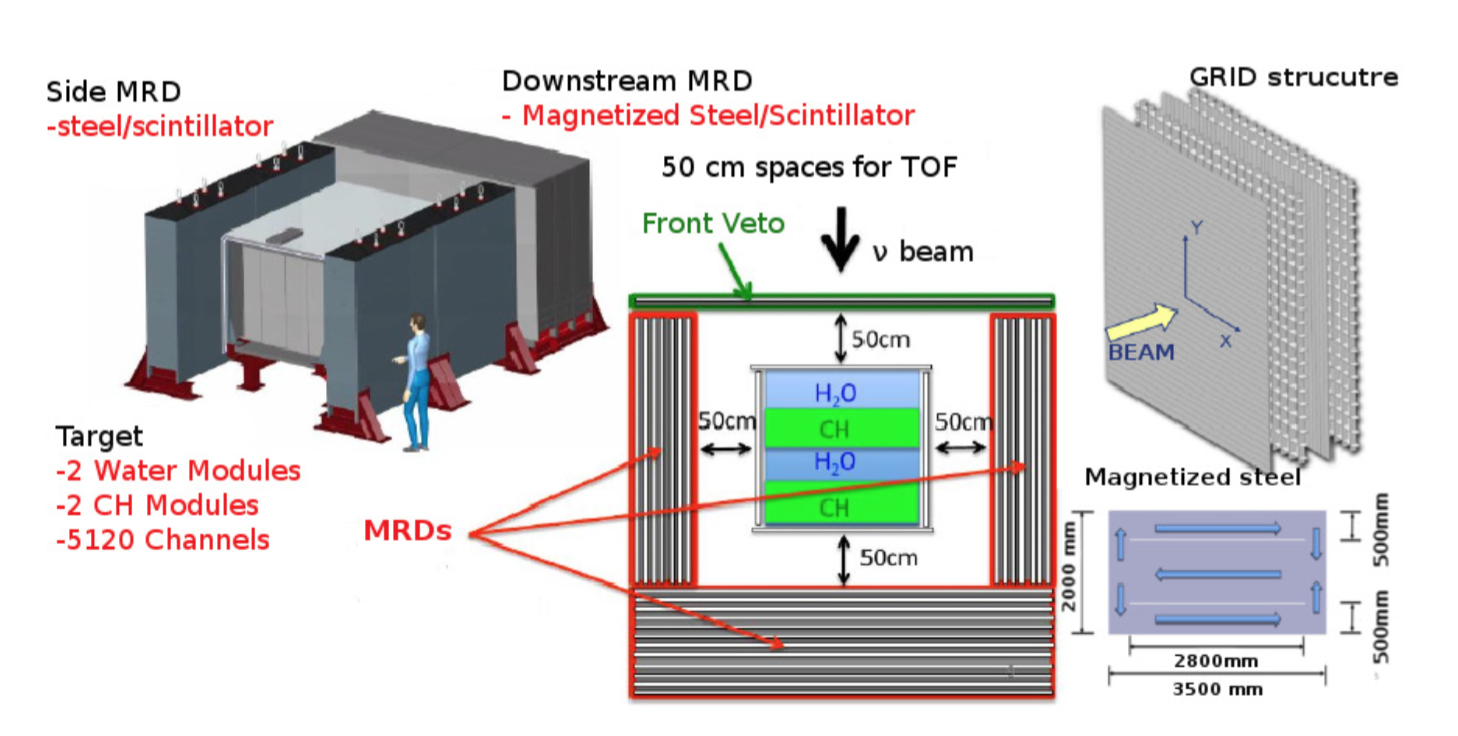
\includegraphics[width=\textwidth]{figures/WAGASCI.png}
\caption{The basic structure of the WAGASCI detector including one of the possible designs for the MIND plates.~\cite{30WAGASCI}.}
\label{fig:WAGASCI}
\end{figure}


\subsection{Collaboration}
No idea, is there even an official website?
\subsection{Layout}
Official images?
\subsection{Motivation}
Official paper?

\section{BabyMIND}
\subsection{Collaboration}
Do we have an official list?
\subsection{Layout}
What papers, images can I should I use.
\subsection{Motivation}
In the white paper? LOI.